\section{Bifurcations}

This section lists the bifurcations that happen at the borders of ``type A'' and ``type B'' parameter regions, respectively.
\Cref{fig:final.regions.whole.halved} shows the borders of the period regions in full.
\Cref{fig:final.regions.CandD16.halved} is a zoomed-in version, that pictures the two regions that this section investigates.
These two regions are $\P_{\A^5\B^3C^5\D^3}$, which is the parameter region that includes the point $C_{16}$, and $\P_{\A^5\B^3\C^4\D^4, \A^4\B^4\C^5\D^3}$, which includes the point $D_{16}$.
The arrows in that figure mark, where the bifurcation diagrams in this section are computed.

\begin{figure}
    \centering
    \begin{subfigure}{0.4\textwidth}
        \centering
        \includegraphics[width=\textwidth]{60_Final/2D_Regions_Whole/result-halved.png}
        \caption{Complete Parameter Region}
        \label{fig:final.regions.whole.halved}
    \end{subfigure}
    \begin{subfigure}{0.4\textwidth}
        \centering
        \includegraphics[width=\textwidth]{60_Final/2D_Regions_CandD16/result-halved.png}
        \caption{Only showing $C_{16}$ and $D_{16}$}
        \label{fig:final.regions.CandD16.halved}
    \end{subfigure}
    \caption{2D Period Regions of Halved Final Model}
\end{figure}

\subsection{``Type'' A Parameter Regions}

We start with the bifurcations bounding the ``type A'' parameter region of the point $C_{16}$.
The borders are enumerated as $C_{16}^\uparrow, C_{16}^\rightarrow, C_{16}^\downarrow,$ and $C_{16}^\leftarrow$, where the arrow in the superscript indicates the side of the border.
So $C_{16}^\uparrow$ means the upper border of the period region, that contains the point $C_{16}$.

\subsubsection{The Boundary $C_{16}^\uparrow$}

When scanning across the upper border of this parameter region, one gets the figure \Cref{fig:final.bifurcation.C.up}
It is not immediately clear, what kind of bifurcation happens.
The bifurcation diagram has to be read from left to right, this is also true for all other bifurcation diagrams in this section.
We are interested in what happens to the stable cycle that exists at the start and causes it to vanish.
The cycle is near the border $\A\B$ when it vanishes, so we can zoom into that area.
It is marked red in the bifurcation diagram and pictured in \Cref{fig:bifurcation.C.up.zoomed}.
It is immediately clear, that this is a border bifurcation with the stable cycle $\A^5\B^3\C^5\D^3$ colliding with the border $d_1$ from the left side, meaning one point on the branch $\A$ collides with this border.
We will write $\BCB_{d_1, d_3}^{\A^5\B^3\C^5\D^3, r}$, which means that this is a border bifurcation at the border $d_1$ and $d_3$ where the points collide from the left (branches $\A$ and $\C$ respectively).

\begin{figure}
    \centering
    \begin{subfigure}{0.4\textwidth}
        \centering
        \includegraphics[width=\textwidth]{60_Final/1D_Bif_LCU16/result.png}
        \caption{Complete}
        \label{fig:final.bifurcation.C.up}
    \end{subfigure}
    \begin{subfigure}{0.4\textwidth}
        \centering
        \includegraphics[width=\textwidth]{60_Final/1D_Bif_LCU16_Zoomed/result.png}
        \caption{Zoomed in at Border $\A\B$}
        \label{fig:bifurcation.C.up.zoomed}
    \end{subfigure}
    \caption{1D Bifurcation Diagrams of $C_{16}^\uparrow$}
\end{figure}

\subsubsection{The Boundary $C_{16}^\rightarrow$}

$BB_{\B\C}^\leftarrow \land BB_{\D\A}^\leftarrow$ at the same time.

\begin{figure}
    \centering
    \begin{subfigure}{0.4\textwidth}
        \centering
        \includegraphics[width=\textwidth]{60_Final/1D_Bif_LCR16/result.png}
        \caption{Complete}
        \label{fig:final.bifurcation.C.right}
    \end{subfigure}
    \begin{subfigure}{0.4\textwidth}
        \centering
        \includegraphics[width=\textwidth]{60_Final/1D_Bif_LCR16_Zoomed/result.png}
        \caption{Zoomed in at Border $\B\C$}
        \label{fig:final.bifurcation.C.right.zoomed}
    \end{subfigure}
    \caption{1D Bifurcation Diagrams of $C_{16}^\rightarrow$}
\end{figure}

\subsubsection{The Boundary $C_{16}^\downarrow$}

$BB_{\A\B}^\leftarrow \land BB_{\C\D}^\leftarrow$ at the same time.

\begin{figure}
    \centering
    \begin{subfigure}{0.4\textwidth}
        \centering
        \includegraphics[width=\textwidth]{60_Final/1D_Bif_LCD16/result.png}
        \caption{Complete}
        \label{fig:final.bifurcation.C.down}
    \end{subfigure}
    \begin{subfigure}{0.4\textwidth}
        \centering
        \includegraphics[width=\textwidth]{60_Final/1D_Bif_LCD16_Zoomed/result.png}
        \caption{Zoomed in at Border $\A\B$}
        \label{fig:final.bifurcation.C.down.zoomed}
    \end{subfigure}
    \caption{1D Bifurcation Diagrams of $C_{16}^\downarrow$}
\end{figure}

\subsubsection{The Boundary $C_{16}^\leftarrow$}

$BB_{\B\C}^\rightarrow \land BB_{\D\A}^\rightarrow$ at the same time.

\begin{figure}
    \centering
    \begin{subfigure}{0.4\textwidth}
        \centering
        \includegraphics[width=\textwidth]{60_Final/1D_Bif_LCL16/result.png}
        \caption{Complete}
        \label{fig:final.bifurcation.C.left}
    \end{subfigure}
    \begin{subfigure}{0.4\textwidth}
        \centering
        \includegraphics[width=\textwidth]{60_Final/1D_Bif_LCL16_Zoomed/result.png}
        \caption{Zoomed in at Border $\B\C$}
        \label{fig:final.bifurcation.C.left.zoomed}
    \end{subfigure}
    \caption{1D Bifurcation Diagrams of $C_{16}^\leftarrow$}
\end{figure}

\subsection{``Type B'' Parameter Regions}

\subsubsection{The Boundary $D_{16}^\uparrow$}

$\A^5\B^3\C^4\D^4$: $BB_{\A\B}^\rightarrow$ \\
$\A^4\B^4\C^5\D^3$: $BB_{\C\D}^\rightarrow$

\begin{figure}
    \centering
    \begin{subfigure}{0.4\textwidth}
        \centering
        \includegraphics[width=\textwidth]{60_Final/1D_Bif_LDU16/result.png}
        \caption{Complete}
        \label{fig:final.bifurcation.D.up}
    \end{subfigure}
    \begin{subfigure}{0.4\textwidth}
        \centering
        \includegraphics[width=\textwidth]{60_Final/1D_Bif_LDU16_Zoomed/result.png}
        \caption{Zoomed in at Border $\A\B$}
        \label{fig:final.bifurcation.D.up.zoomed}
    \end{subfigure}
    %\begin{subfigure}{0.3\textwidth}
    %    \centering
    %    \includegraphics[width=\textwidth]{60_Final/Cobweb_LDU16/result.png}
    %    \caption{Cobweb at Bifurcation}
    %    \label{fig:final.bifurcation.D.up.cobweb}
    %\end{subfigure}
    \caption{1D Bifurcation Diagrams and Cobweb of $D_{16}^\uparrow$}
\end{figure}

\subsubsection{The Boundary $D_{16}^\rightarrow$}

$\A^5\B^3\C^4\D^4$: $BB_{\D\A}^\leftarrow$ \\
$\A^4\B^4\C^5\D^3$: $BB_{\B\C}^\leftarrow$

\begin{figure}
    \centering
    \begin{subfigure}{0.4\textwidth}
        \centering
        \includegraphics[width=\textwidth]{60_Final/1D_Bif_LDR16/result.png}
        \caption{Complete}
        \label{fig:final.bifurcation.D.right}
    \end{subfigure}
    \begin{subfigure}{0.4\textwidth}
        \centering
        \includegraphics[width=\textwidth]{60_Final/1D_Bif_LDR16_Zoomed/result.png}
        \caption{Zoomed in at Border $\B\C$}
        \label{fig:final.bifurcation.D.right.zoomed}
    \end{subfigure}
    %\begin{subfigure}{0.3\textwidth}
    %    \centering
    %    \includegraphics[width=\textwidth]{60_Final/Cobweb_LDR16/result.png}
    %    \caption{Cobweb at Bifurcation}
    %    \label{fig:final.bifurcation.D.right.cobweb}
    %\end{subfigure}
    \caption{1D Bifurcation Diagrams and Cobweb of $D_{16}^\rightarrow$}
\end{figure}

\subsubsection{The Boundary $D_{16}^\downarrow$}

$\A^5\B^3\C^4\D^4$: $BB_{\C\D}^\leftarrow$ \\
$\A^4\B^4\C^5\D^3$: $BB_{\A\B}^\leftarrow$

\begin{figure}
    \centering
    \begin{subfigure}{0.4\textwidth}
        \centering
        \includegraphics[width=\textwidth]{60_Final/1D_Bif_LDD16/result.png}
        \caption{Complete}
        \label{fig:final.bifurcation.D.down}
    \end{subfigure}
    \begin{subfigure}{0.4\textwidth}
        \centering
        \includegraphics[width=\textwidth]{60_Final/1D_Bif_LDD16_Zoomed/result.png}
        \caption{Zoomed in at Border $\A\B$}
        \label{fig:final.bifurcation.D.down.zoomed}
    \end{subfigure}
    %\begin{subfigure}{0.3\textwidth}
    %    \centering
    %    \includegraphics[width=\textwidth]{60_Final/Cobweb_LDD16/result.png}
    %    \caption{Cobweb at Bifurcation}
    %    \label{fig:final.bifurcation.D.down.cobweb}
    %\end{subfigure}
    \caption{1D Bifurcation Diagrams and Cobweb of $D_{16}^\downarrow$}
\end{figure}

\subsubsection{The Boundary $D_{16}^\leftarrow$}

$\A^5\B^3\C^4\D^4$: $BB_{\D\A}^\rightarrow$ \\
$\A^4\B^4\C^5\D^3$: $BB_{\B\C}^\rightarrow$

\begin{figure}
    \centering
    \begin{subfigure}{0.4\textwidth}
        \centering
        \includegraphics[width=\textwidth]{60_Final/1D_Bif_LDL16/result.png}
        \caption{Complete}
        \label{fig:final.bifurcation.D.left}
    \end{subfigure}
    \begin{subfigure}{0.4\textwidth}
        \centering
        \includegraphics[width=\textwidth]{60_Final/1D_Bif_LDL16_Zoomed/result.png}
        \caption{Zoomed in at Border $\B\C$}
        \label{fig:final.bifurcation.D.left.zoomed}
    \end{subfigure}
    %\begin{subfigure}{0.3\textwidth}
    %    \centering
    %    \includegraphics[width=\textwidth]{60_Final/Cobweb_LDL16/result.png}
    %    \caption{Cobweb at Bifurcation}
    %    \label{fig:final.bifurcation.D.left.cobweb}
    %\end{subfigure}
    \caption{1D Bifurcation Diagrams and Cobweb of $D_{16}^\leftarrow$}
\end{figure}
